\subsubsection{Chi quadro residui}

Come prima, usiamo nuovamente il test del $\chi^2$ per valutare le incertezze. Come già ripetuto più volte,
le incertezze sono sottostimate e quindi vogliamo fare il test del chi quadro, il cui risultato non sarà compatibile con il valor atteso,
e poi lo useremo per aggiustare gli errori.

I valori attesi $\nu \equiv \chi\ped{teo}^2$, per ciascuna sottoserie di dati, sono uguali al numero di gradi di libertà,
ovvero al numero di dati $N_j$ del gruppo $j$-esimo meno due, che è il numero di parametri calcolati con la regressione.
L'incertezza $\delta \nu$ si calcola con la formula $\delta \nu = \sqrt{2\nu}$. Anticipiamo inoltre che prendiamo un fattore di copertura
$k = 3$.

Si è calcolato il $\chi^2$ con la formula (\ref{eq:chi2}) del paragrafo \ref{chi_1}.
La seguente tabella riporta i valori attesi per ogni gruppo, con relative incertezze ed anche i corrispondenti valori del chi quadro.

\begin{center}
    \begin{tabular}{l c c c c}
        \multicolumn{5}{c}{\textbf{Valori teorici del $\chi^2$}} \\
        \toprule
        & Gruppo 1 & Gruppo 2 & Gruppo 3 & Gruppo 4 \\
        \midrule
        $N_j$ & 7 & 14 & 11 & 12 \\
        $\nu$ & 5 & 12 & 9 & 10 \\
        $\delta \nu$ & 3 & 5 & 4 & 4 \\
        $\chi^2$ & 159 & 1521 & 3587 & 1541 \\
        \bottomrule
    \end{tabular}
\end{center}

Osserviamo immediatamente che nessuno dei valori del chi quadro è compatibile con il suo valore teorico entro l'intervallo di confidenza.
Come atteso, è necessario aggiustare le incertezze, tuttavia i valori del $\chi^2$ sono significativamente più bassi rispetto a
quelli ottenuti prima di dividere i dati in sottoserie.

L'aggiustamento delle incertezze si svolge come già spiegato nel paragrafo \ref{chi_1} con la formula (\ref{eq:corr_err}).
Il calcolo dell'incertezza sulla temperatura si svolge come indicato nella formula (\ref{eq:corr_err_theta}).
Svolgendo la procedura si ottengono le seguenti incertezze corrette sulla temperatura. Sono riportate le incertezze corrette
sul dislivello per completezza.

\begin{center}
    \begin{tabular}{l c c c c}
        \multicolumn{5}{c}{\textbf{Incertezze corrette sulla temperatura}} \\
        \toprule
        & Gruppo 1 & Gruppo 2 & Gruppo 3 & Gruppo 4 \\
        \midrule
        $\delta d\ped{corr}$ [cm] & 0.2 & 0.5 & 0.9 & 0.5 \\
        $\delta \theta\ped{corr}$ [\si{\celsius}] & 0.07 & 0.12 & 0.19 & 0.14 \\
        \bottomrule
    \end{tabular}
\end{center}

Ora queste incertezze ci sembrano molto più realistiche di quelle ricavate in precedenza, infatti, a parte l'incertezza del 
gruppo 3 che è ancora piuttosto cospicua, sono tutte attorno a \SI{0.10}{\celsius}. Notiamo anche che
l'errore sui gruppi 3 e 4 sono più alti, come era possibile aspettarsi.
Nella seconda serie di dati c'è infatti un errore sistematico per il quale le pressioni in salita sono minori di quelle in discesa.

Nonostante la presenza di questo errore, abbiamo deciso di accettare le incertezze che abbiamo qui calcolato, in quanto
sono sicuramente migliori delle incertezze di risoluzione accettate in origine.

Dopo aver corretto le incertezze occorre eseguire nuovamente i fit sui gruppi di dati, per ottenere le nuove incertezze sui parametri
$A$ e $B$. Eseguendo nuovamente il metodo dei minimi quadrati con le nuove incertezze si ottengono i seguenti dati.

\begin{center}
    \begin{tabular}{l c c c c}
        \multicolumn{5}{c}{\textbf{Incertezze corrette su $A$ e $B$}} \\
        \toprule
        & Gruppo 1 & Gruppo 2 & Gruppo 3 & Gruppo 4 \\
        \midrule
        $\delta A$ [cm] & 0.77 & 0.26 & 1.65 & 0.39 \\
        $\delta B$ [\si{\centi\metre\per\celsius}] & 0.04 & 0.03 & 0.08 & 0.04 \\
        \bottomrule
    \end{tabular}
\end{center}

Gli errori sono tutti circa un ordine di grandezza maggiore di quanto stimato in precedenza.

\begin{SCfigure}[][!b]
    \centering
    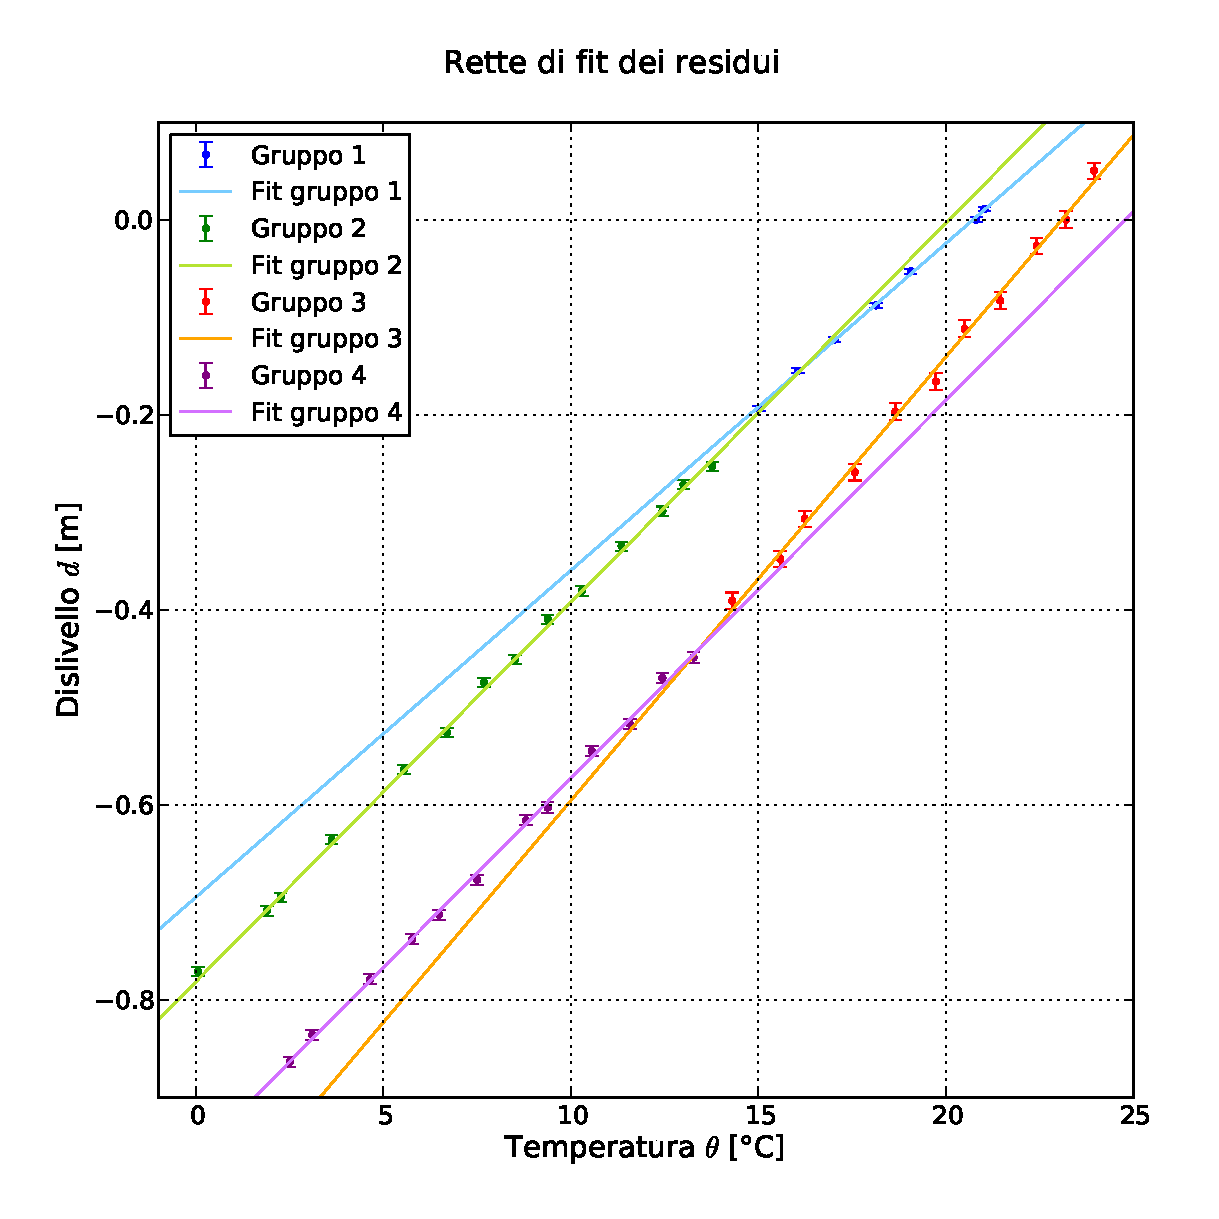
\includegraphics[width=120mm]{immagini/residui.pdf}
    \caption{Il grafico riporta visivamente le quattro regressioni eseguite sui gruppi di dati.
    Le rette si adattano ai dati in maniera sensibilmente migliore di quanto non succedesse prima
    di creare le sottoserie. Le incertezze riportate sono gli errori sul dislivello corretti, diversi
    da gruppo a gruppo. I gruppi di dati e le relative rette sono indicati con colori simili per
    aumentare la chiarezza del grafico.}
    \label{fig:residui}
\end{SCfigure}

\begin{figure}[p]
    \centering
    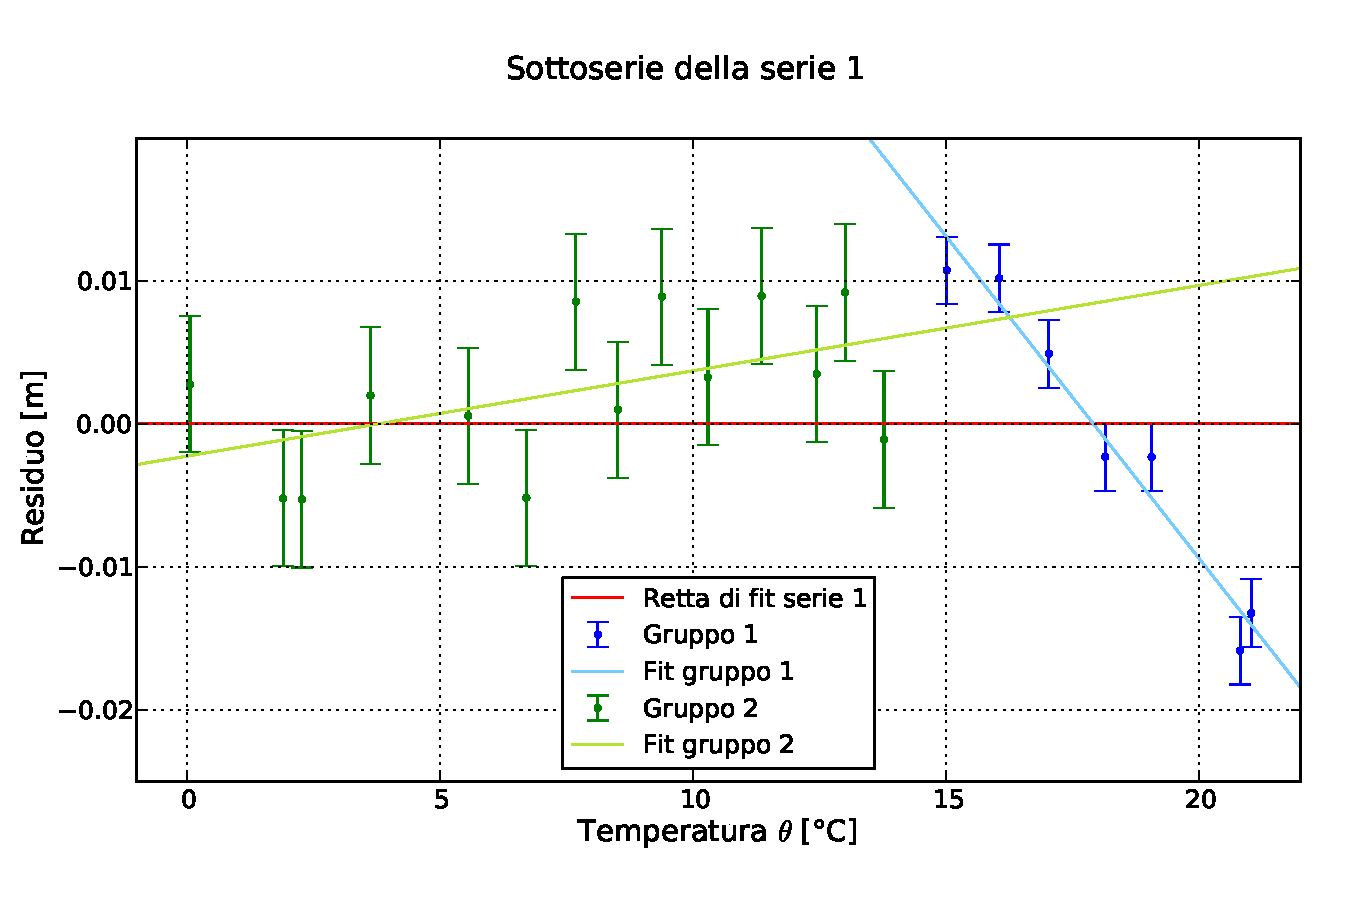
\includegraphics[width=130mm]{immagini/fit1r.pdf}
    \caption{Dettaglio dei residui della prima serie. Il grafico è analogo a quello in figura \ref{fig:fit1},
    solo che qui sono evidenziati i gruppi 1 e 2, ricavati dalla prima serie, che sono
    riportati con colori ed incertezze diverse. È stato inoltre tolto un punto.
    I colori sono uguali a quelli della Figura \ref{fig:residui},
    per facilitare il confronto, mentre le incertezze riportate sono le incertezze corrette sul dislivello.}
    \label{fig:fit1r}
\end{figure}

\begin{figure}[p]
    \centering
    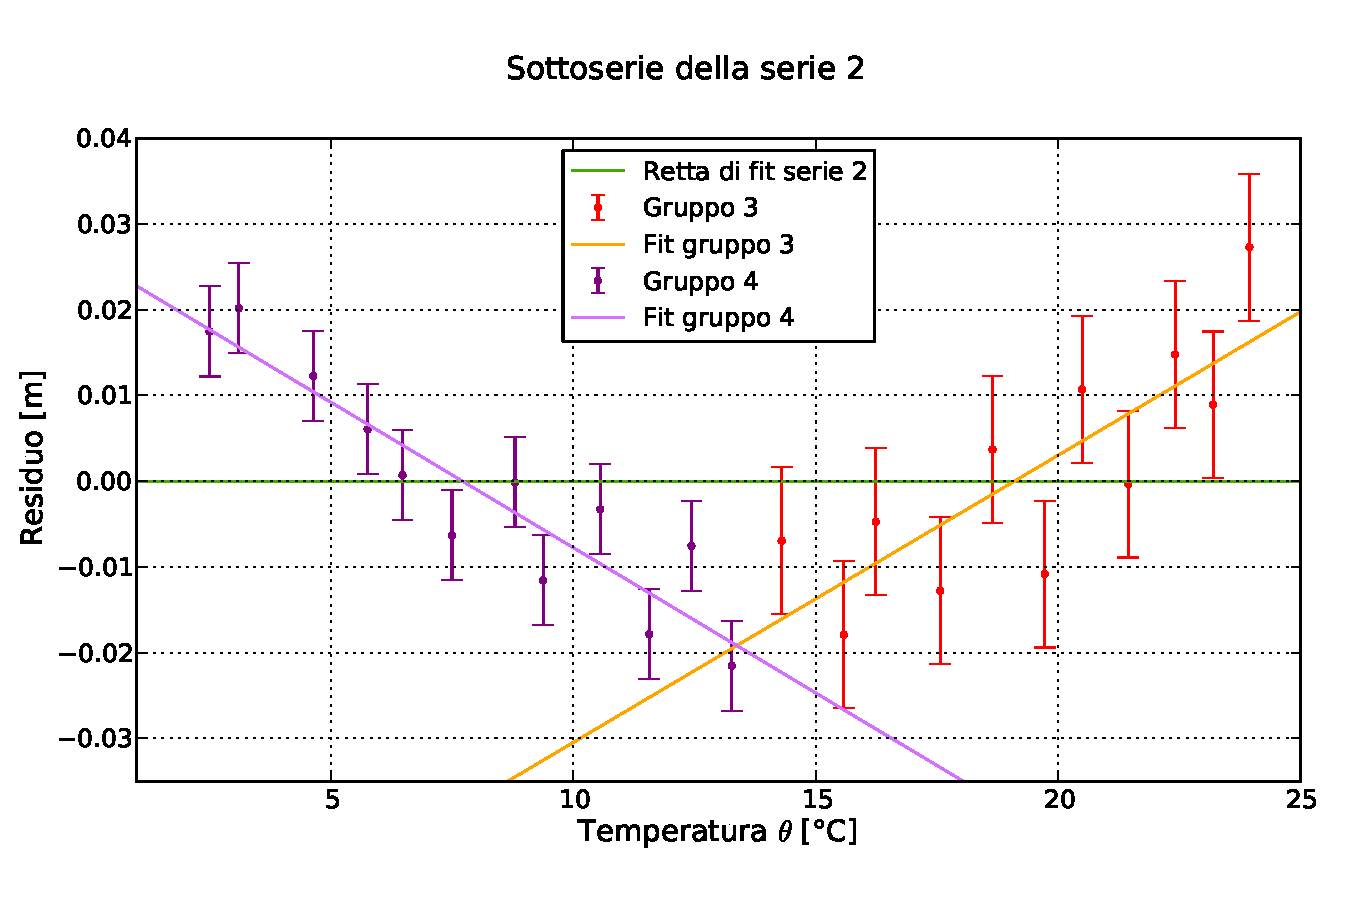
\includegraphics[width=130mm]{immagini/fit2r.pdf}
    \caption{Analogamente all'immagine precedente, questo plot è simile a quello in Figura \ref{fig:fit2},
    tranne che sono graficati distintamente i punti dei gruppi 3 e 4. Le barre d'errore indicano le incertezze
    corrette sul dislivello.}
    \label{fig:fit2r}
\end{figure}
